%!TEX root = ../../../main.tex

\subsection{Context Diagrams}

At this level we define and represent the different systems. This allows us to visualize the systems interactions with other external systems.

\begin{figure}[H]
\centering
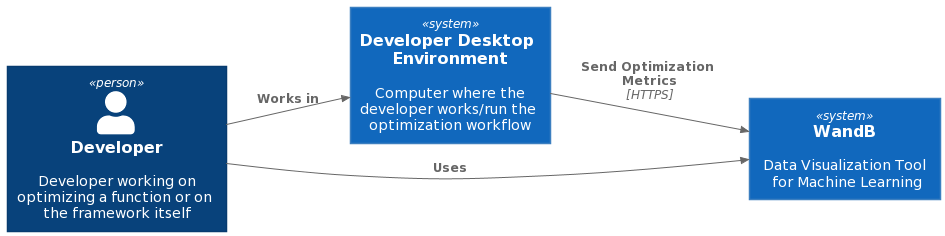
\includegraphics[width=\textwidth]{images/c1_new.png}
\caption{Level 1: System context diagram}
\label{fig:level1}
\end{figure}

As we can see in figure \ref{fig:level1}, the overall working environment consists of the Weight and Biases tooling, provided as an online service, the CAM2 software, responsible for executing the actual optimizable algorithm, and a Python environment, containing the Ray Tune framework, the developed tooling and any changes the privileged developer decides to apply to the optimizing process.

\subsection{Container Diagrams}

At this level we define and represent the different \textit{containers} in the system. We have previously referred to containerization systems such as Docker, but in this case we are referring to containers as a defined software unit, such as a database or a web app.

%http://www.plantuml.com/plantuml/png/jLBDRjim3BxxAJYV4c1jq6AddPgsmpQWnOB-RCU2iPXOg4ng4fqiBVRkanmbMu1Wj-OIa_v-I7w-Y8f1-yvLxomthZS4hQgF7oUJWElJfTMsd_UHGYEin7hQI3Vn3ZbpJg8QP-UJgmydiznwlBsPT1YLGcezNMN6BptrRwQEbYcycNxdXOdB_8uM2YeGxB9LC3PGerQugcOKel383tzJPp6-X_gQLkGazUf_2rXBUBQy1CiWNcrdNtA5iEXvKAl7LNM_YKhTqwNqR31iHl7iGEAQuhEAXq-yia6u8zPw_5fLa7xxaupyXdYLUBEDji87uDGjk0Ze7FWjH4LScdmHiACy9Y0RCCNMG2E6ydI7DWrsvrblUdkUTNzODhAECFNUsGQ7ZSfhYBBGDOOiyll8akUPdYmlwp6y5fTo_z4wzUVexGu2qzdNmOxcsyVwZXgoAuh3q3v8Gp6cIbi2WuffA-c6gbnz66q7hCV7_FPcdn_tPdECPE0QOpiN36R8Dij_jx57jvDz476ma02tsBIM2Mu80wUWjwlVaJlyM8RT7oF5dSrVW_4Hz5b6fO0YM2w0adPE8z_YPqzHOIQM5QwSz0OITrdIhxyyFCmARnlVbbtV4vl3--JJ5SAXqJwG_vFk4skWxV6mFMtzBIoHxKj9nx8AQB3eSXONIRBlt1y0

\begin{figure}[h]
\centering
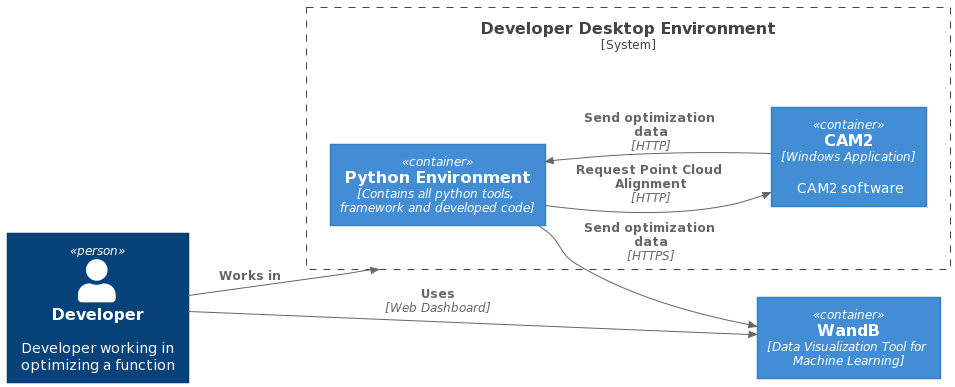
\includegraphics[width=\textwidth, keepaspectratio]{images/c2_new.png}
\caption{Level 2: Container diagram}
\label{fig:level2}
\end{figure}

As we can see in figure \ref{fig:level2} all of the development took place within the Python environment as the Ray Tune and WandB are services that were integrated into the developed code. All communication between each container and system uses HTTP in the form of APIs (CAM2 API, WandB logger API). Finally, the developer can analyse the results of the optimization process in the WandB \acrfull{gui}.

\subsection{Component Diagrams}

At this level we define and represent the different \textit{components} in the system. These components are important parts of a given container, such as controllers or services. 

We split components into their respective system or container.

The \acrshort{python} development environment is divided into 5 components: CAM2 HTTP interface, Search Algorithms, Search Spaces, Ray Tune and the WandB Logger for Ray Tune.


\begin{figure}[H]
\centering
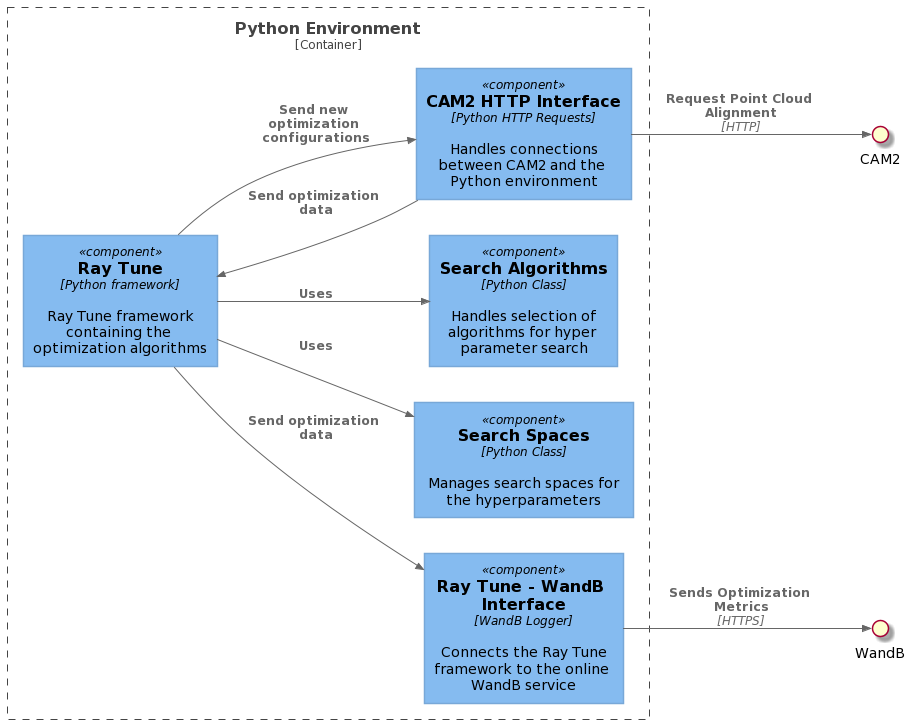
\includegraphics[width=0.75\textwidth]{images/c3_python.png}
\caption{Level 3: Python Environment Component Diagram}
\label{fig:l3_python}
\end{figure}

The CAM2 container was treated throughout the development cycle as a black box, without any direct access to its codebase, only its \acrfull{api}. From information provided by the CAM2 development team, we were able to define 2 components within the CAM2 container: the included web server and the rest of the CAM2 software.

\begin{figure}[H]
\centering
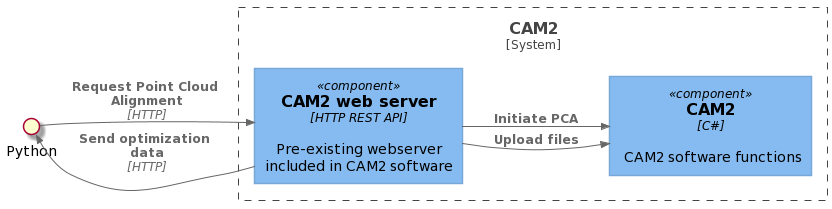
\includegraphics[width=0.75\textwidth]{images/c3_cam2.png}
\caption{Level 3: CAM2 Component Diagram}
\label{fig:l3_cam2}
\end{figure}

Similarly, the WandB container was treated throughout the development cycle as a black box, with access only to its \acrfull{api} and \acrshort{ui}. From the usage of the service throughout the internship we can ascertain two different components: the Weight \& Biases \acrshort{api} and web dashboard.

\begin{figure}[H]
\centering
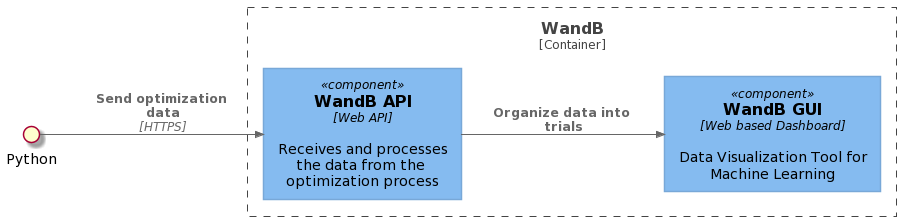
\includegraphics[width=0.75\textwidth]{images/c3_wandb.png}
\caption{Level 3: WandB Component Diagram}
\label{fig:l3_wandb}
\end{figure}

\subsection{Code Diagrams}

The Ray Tune framework contains various classes, both available to be edited by a privileged developer as well as static classes.

\begin{figure}[H]
\centering
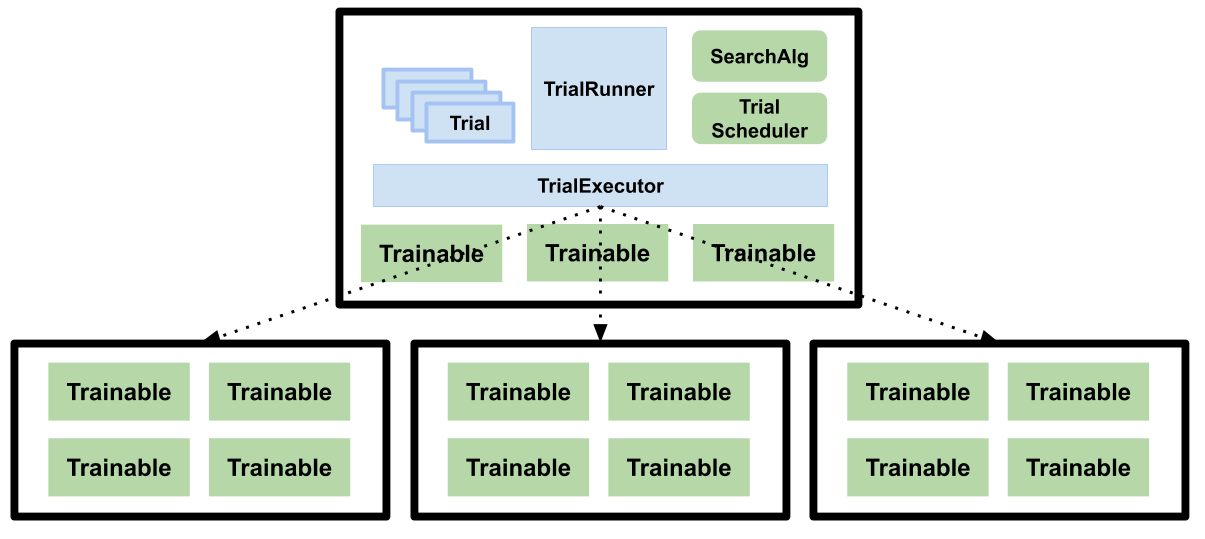
\includegraphics[width=0.75\textwidth, keepaspectratio]{images/tune_component.png}
\caption{Level 4: Ray Tune Class Diagram \parencite{ray}}
\label{fig:l3_ray}
\end{figure}

As we can see in figure \ref{fig:l3_ray}, the Ray Tune framework contains internal components (blue boxes) and public-facing components (green boxes) \parencite{ray}. Tune’s main components consist of TrialRunner, Trial objects, TrialExecutor, SearchAlg, TrialScheduler, and Trainable. Of these, only the Trainable was edited for this project, although there is support for new algorithm development, which is not within the scope of this project.

We can also see in figure \ref{fig:l3_ray_seq} how the different components interact with each other during the optimization process. Although this was not directly developed within this internship, it was extensively used throughout.

\begin{sidewaysfigure}
\centering
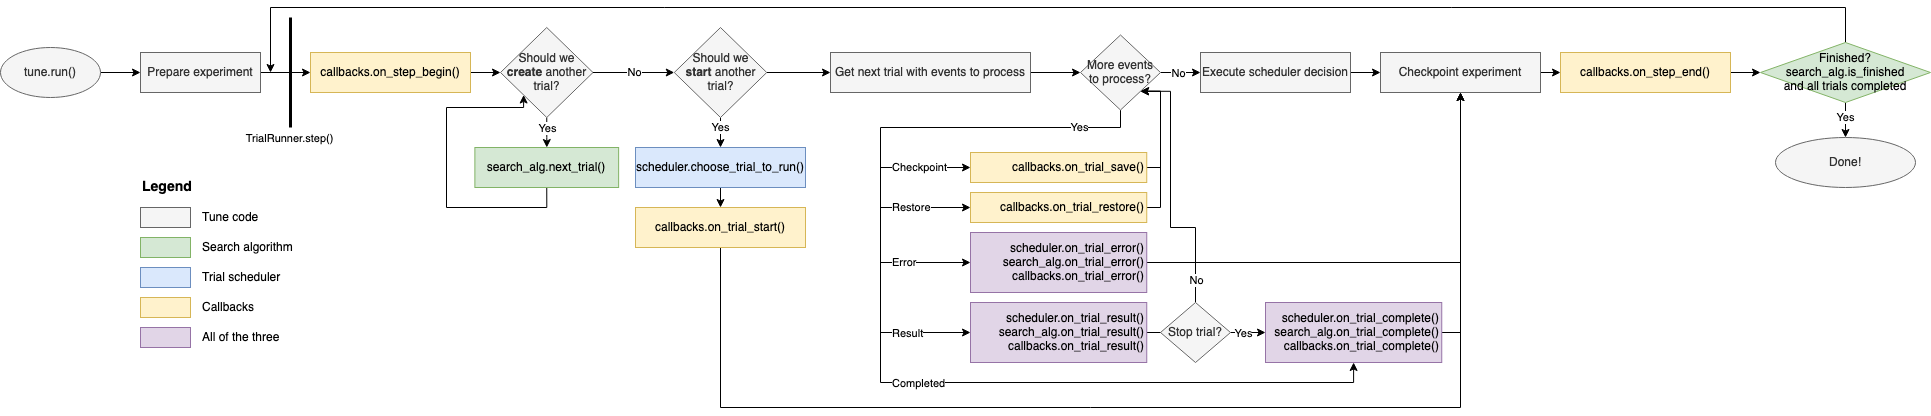
\includegraphics[width=\textwidth, keepaspectratio]{images/tune_component_flwo.png}
\caption{Level 4: Ray Tune Sequence Diagram \parencite{ray}}
\label{fig:l3_ray_seq}
\end{sidewaysfigure}